\section{Background}
\label{background}
%\subsection{Terminologies}
This work focuses on the
event extraction task proposed by the Automatic Content Extraction (ACE) program \cite{doddington2004automatic} which
defines the following terminologies for event extraction:

\begin{itemize}
	\item \textbf{Event mention}:  a phrase or sentence within which an event is described, including a trigger and its arguments.
	\item \textbf{Event trigger}: the main word or phrase that most clearly expresses the occurrence of an event. An event trigger is typically a verb or a noun in the ACE framework.
	\item \textbf{Event argument}: an entity, temporal expression or value that is involved in an event.
	\item \textbf{Argument role}: the relationship between an argument and the event in which it participates.
\end{itemize}

Specifically, in the initial 2005 evaluation, there are three languages in the ACE event extraction task,  English, Chinese and Arabic. Similar to many other NLP tasks, English event extraction receives relatively more attention in the literature, while Chinese and Arabic are not in the spotlight.  In this paper, we aim to improve Chinese event extraction.

Despite of the differences among these three languages, their ACE task setups remain the same.
Given a text document, an event extraction system need to identify all event triggers with specific types and their corresponding arguments for each sentence. For example, given an example sentence, S1, in Chinese, the system should produce a structured output, including a typed event trigger  and its corresponding arguments  with pre-defined  roles, as shown in Figure~\ref{exfigure}.

\begin{figure}
\centering
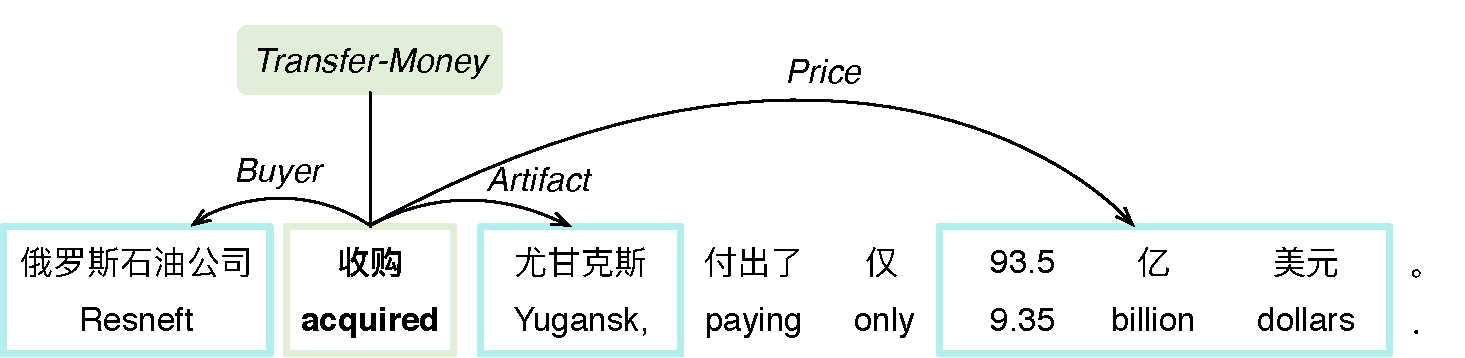
\includegraphics[width=.9\textwidth]{example.pdf}
\caption{An example of Chinese event extraction for S1, where English translations are provided besides the Chinese words. The example sentence has one \emph{Transfer-Money} event mention triggered by \textit{收购 (acquired)}, which have three arguments, \textit{俄罗斯石油公司 (Rosneft)} as the \emph{Transfer-Money} event's \textit{Buyer}, \textit{尤甘斯克 (Yugansk)}  as its \textit{Artifact}, and \textit{93.5 亿美元 (9.35 billion dollars)} as its \textit{Price}.}
\label{exfigure}
\end{figure}

\begin{quote}
S1: 俄罗斯石油公司 \hspace{0.3cm}收购 \hspace{0.3cm}尤甘斯克 \hspace{0.3cm}付出 \hspace{0.2cm}了 \hspace{0.2cm}仅 \hspace{0.3cm}93.5 \hspace{0.3cm}亿 \hspace{0.3cm}美元。

\hspace{0.52cm} Rosneft acquired Yugansk, paying only 9.35 billion dollars.
\end{quote}

To produce such a structured output, a system usually has to solve the following four subtasks,
\begin{enumerate}
	\item \textbf{Trigger identification}: recognize the event trigger from the sentence, e.g., \textit{``收购'' (acquired)} should be identified as a trigger of an event;
	\item \textbf{Trigger classification}: assign an event type for the identified trigger, e.g., \textit{``收购'' (acquired)} should be assigned with the type \emph{Transfer-Money};
	\item \textbf{Argument identification}: determine whether a word or phrase plays a certain role in the event mention, e.g., \textit{``俄罗斯石油公司'' (Rosneft)}, \textit{``尤甘斯克'' (Yugansk)}, and \textit{``93.5亿美元'' (9.35 billion dollars)} are the arguments of this \emph{Transfer-Money} event;
	\item \textbf{Argument classification}: assign a role to each identified argument, e.g., \textit{``俄罗斯石油公司'' (Rosneft)}, \textit{``尤甘斯克'' (Yugansk)}, and \textit{``93.5亿美元'' (9.35 billion dollars)} play the roles of \emph{Buyer}, \emph{Artifact} and \emph{Price}, respectively, in this  \emph{Transfer-Money} event.
\end{enumerate}


However, such a 4-step pipeline system inevitably suffers from the error propagation problems, let alone language specific challenges,  e.g., Chinese word segmentation, and insufficient capability of existing NLP tools for those low-resourced languages.  As addressed in the literature \cite{chen2009language,li2012employing}, errors made by an upstream subtask, e.g., Chinese word segmentation or trigger identification,  will propagate to the downstream subtasks, e.g., tigger classification or argument identification, and could adversely affect their performance. In most cases, downstream subtasks will have no chance to even alleviate such effect. The work presented in \cite{chen2012joint} addresses the issue by recasting the 4-step framework  into two joint learning tasks, namely, \textbf{trigger labeling} and \textbf{argument labeling}. The  former jointly learns trigger identification and classification, while the latter learns argument identification and argument classification simultaneously, which has been shown to be promising in Chinese event extraction~\cite{chen2012joint}. In this work, we follow this 2-step approach for Chinese event extraction. 


Previous state-of-the-art approaches in Chinese event extraction~\cite{chen2009language,li2012employing,chen2012joint,li2013joint} usually rely on a variety of elaborate features, which, in general, must be designed by experts, and extracted using lexical or syntactic analysis tools. Those features can be roughly divided into two categories: \textbf{lexical features} and \textbf{sentence-level features}. The former are designed to capture local features, while the latter characterize global topics of the sentences.  Take trigger labeling in the following sentences as an example: the target word \textit{``成立'' (found)} indicates a \emph{Business} event in S2, but not in either S3 or S4.

\begin{quote}
S2: Intel 在 中国 \textbf{成立} 了 研究中心。

\hspace{0.52cm} Intel \textbf{founds} a research center in China.
\end{quote}

\begin{quote}
S3: 它 \textbf{成立} 于 1994 年 , 现在 是 一支 深 受 欢迎 的 乐队。

\hspace{0.52cm} It was \textbf{founded} in 1994, and now is a very popular band.
\end{quote}

\begin{quote}
S4: 医院 已 \textbf{成立} 救援中心。

\hspace{0.52cm} The hospital has \textbf{founded} rescue centers.
\end{quote}

\textbf{Lexical features}, often in the form of word lemma or part-of-speech tags (POS), provide semantic information of a candidate word and its surrounding context. In S4, the neighboring word ``救援中心''(rescue center) serves as a lexical feature for \textit{``成立'' (found)}, indicating a medical institute,  thus we can infer that \textit{``成立'' (found)} is not a trigger of a \emph{Business} event.

\textbf{Sentence-level features} are usually extracted from syntactic structures, and  maintain important clues about the whole sentence. S3 talks about ``它\_是\_乐队'' (it\_is\_band) and ``它\_成立\_1994'' (it\_founded\_1994), indicating the verb ``成立'' (founded) relates to a musical group, thus should not be regarded as a trigger of a \emph{Business} event.

%\subsection{Problem Scope} 
The aim of this work is to investigate ways to automatically find effective features for \textbf{trigger labeling} and \textbf{argument labeling}.
Although event extraction (mainly argument labeling) also depends on name identification and entity mention co-reference, which are challenging by themselves, these techniques fall out of the scope of this work. In comply with the standard practice in prior work~\cite{chen2009language,chen2012joint}, we directly utilize the entity recognition ground-truth provided by ACE for argument labeling. We stress that other work on improving argument labeling is thus orthogonal to our approach.

%\subsection{Drawbacks of Manual Feature Engineering} 
Traditional event extraction methods \cite{ahn2006stages,chen2009language,li2012employing,chen2012joint} rely on those carefully-designed features to build multi-class classifiers for each subtask. They first apply a series of NLP tools to extract lexical features (e.g., \POS tagging, and named entity recognition (\NER)) and sentence-level features (e.g., dependency parsing, and semantic role labeling (\SRL)). Then in the training stage, they learn to weight each feature for each subtask in the pipeline, independently, with a classifiers, e.g., conditional random fields (\CRF) \cite{lafferty2001conditional}, support vector machines~\cite{suykens1999least}, maximum entropy \cite{phillips2006maximum}, etc. Although those methods can achieve satisfactory performances, they still suffer from the hard feature engineering, where human expert involvement is necessary,  and many semantic/syntactic tools may not work as well as we expected. This is a particular problem for low-resourced languages, for which the overall performance is often below 70\%, resulting in incorrect feature extraction and confusing the classifier.

\begin{quote}
	S5: 犯罪 嫌疑人 都 \textbf{落入 法网}。
	
	\hspace{0.55cm} The suspects were \textbf{arrested}.
\end{quote}
\begin{quote}
	S6: 警察 \textbf{击毙} 了 一名 歹徒。
	
	\hspace{0.55cm} Polices \textbf{shoot} and \textbf{kill} a criminal.
\end{quote}
\begin{quote}
	S7: 这 是 一件 预谋 的 \textbf{凶杀}案。
	
	\hspace{0.55cm} It is a premeditated \textbf{murder} case.
\end{quote}

Take Chinese event extraction systems as an example. Current Chinese systems do not perform as well as their English counterparts. One of the major obstacles, as suggested by \citeN{li2012employing}, is caused by the Chinese word segmentation, a unique preprocessing step for Chinese. Unlike English, Chinese does not have delimiters between words, which makes word segmentation the very first and fundamental step in Chinese event detection. However, we find that word segmentation granularity does have a great impact on the trigger labeling performance. For example, triggers in S5$\sim$S7 cannot be recognized accurately if we simply predict whether a word is an event trigger or not. In S5, the word ``落入法网'' is usually separated into two words, while the gold-standard trigger is ``落入法网'' as a whole; while in S6, ``击毙'', in most cases, is treated as one single word, but actually, the characters ``击'' and ``毙'' are two triggers of different types, the former an \textit{Attack} event and the latter a \textit{Die} event, respectively. As in such a pipeline framework, incorrect trigger labeling will definitely affect downstream argument labeling, whose inputs are highly related to the predicated triggers.

One of the key innovations of our approach is to recast trigger labeling as a sequence labeling task, and further to combine different neural network components to automatically learn feature representations of different levels capturing both local lexical and sentence level characteristics for event extraction. Doing so allows us to  address the Chinese language-specific issues mentioned above, by exploiting the recent breakthrough effectiveness of deep neural networks in natural language modeling, and to alleviate the burden of hard feature engineering and the reliance on external tools or thesauruses. In the reminder of this paper, we will describe how to build such a system in two-step fashion, trigger labeling and argument labeling. 

